\let\negmpace\undefined
\let\negthickspace\undefined
\documentclass[journal]{IEEEtran}
\usepackage[a5paper, margin=10mm, onecolumn]{geometry}
%\usepackage{lmodern} % Ensure lmodern is loaded for pdflatex
\usepackage{tfrupee} % Include tfrupee package
\setlength{\headheight}{1cm} % Set the height of the header box
\setlength{\headsep}{0mm}     % Set the distance between the header box and the top of the text
\usepackage{xparse}
\usepackage{gvv-book}
\usepackage{gvv}
\usepackage{cite}
\usepackage{amsmath,amssymb,amsfonts,amsthm}
\usepackage{algorithmic}
\usepackage{graphicx}
\usepackage{textcomp}
\usepackage{xcolor}
\usepackage{txfonts}
\usepackage{listings}
\usepackage{enumitem}
\usepackage{mathtools}
\usepackage{gensymb}
\usepackage{comment}
\usepackage[breaklinks=true]{hyperref}
\usepackage{tkz-euclide} 
\usepackage{listings}
% \usepackage{gvv}                                        
\def\inputGnumericTable{}                                 
\usepackage[latin1]{inputenc}                                
\usepackage{color}                                            
\usepackage{array}                                            
\usepackage{longtable}                                       
\usepackage{calc}                                             
\usepackage{multirow}                                         
\usepackage{hhline}                                           
\usepackage{ifthen}                                           
\usepackage{lscape}
\renewcommand{\thefigure}{\theenumi}
\renewcommand{\thetable}{\theenumi}
\setlength{\intextsep}{10pt} % Space between text and floats
\numberwithin{equation}{enumi}
\numberwithin{figure}{enumi}
\renewcommand{\thetable}{\theenumi}
\begin{document}
\bibliographystyle{IEEEtran}
\title{Question-6.5.3.7}
\author{EE24BTECH11038 - MALAKALA BALA SUBRAHMANYA ARAVIND}
% \maketitle
% \newpage
% \bigskip
{\let\newpage\relax\maketitle}
\textbf{Question}:
Find the local maxima of the function $\frac{1}{x^2+2}$.\\
\solution \\
\textbf{Theoritical solution:}\\
Given $f\brak{x}=\frac{1}{x^2+2}$
\begin{align}
    \frac{dy}{dx}&=-\frac{-2x}{\brak{x^2+2}^2}=0\\
    \implies x=0\\
    \frac{d^2y}{dx^2} = -\frac{1}{2}\\  
\end{align}
Since $\frac{d^2y}{dx^2}$ is negative and $\frac{dy}{dx}=0$ at x=0\\
Therefore,$f\brak{0}=\frac{1}{2}$ is the maximum value of the function.\\
\textbf{Computational Solution Using Gradient Descent:}\\
To verify the analytical results, we use gradient descent to find the local maximum. \\
Gradient descent for local maximum : \\ 
Start with $x_0=-3$\\
Update the value of x by the following equation. \\
\begin{align}
    x_{n+1}=x_n+\eta \cdot f^{\prime}\brak{x_n}\\
\end{align}
where:
\begin{align}
    \eta=0.1\\
    f^{\prime}\brak{x}=-\frac{2x}{\brak{x^2+2}^2}
\end{align}
\textbf{computational result}\\
Local Maximum  
\begin{align}
    x=0,f\brak{x}=0.5
\end{align}
\begin{figure}[h!]
	\centering
	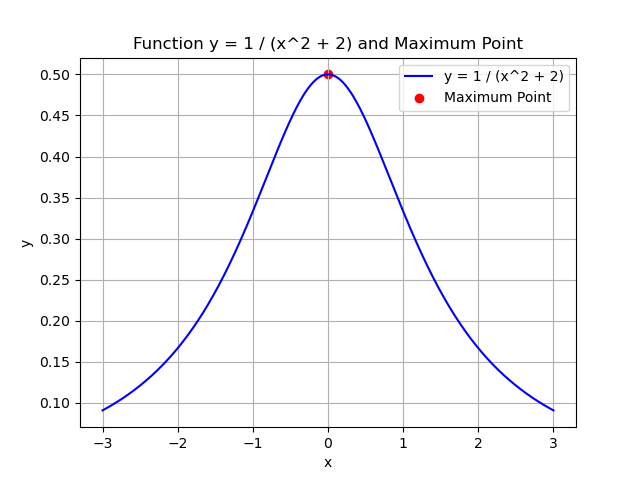
\includegraphics[width=\columnwidth]{figs/Figure_1.png}
	\label{stemplot}
\end{figure}
\end{document}
